% Options for packages loaded elsewhere
\PassOptionsToPackage{unicode}{hyperref}
\PassOptionsToPackage{hyphens}{url}
\PassOptionsToPackage{dvipsnames,svgnames,x11names}{xcolor}
%
\documentclass[
]{article}
\usepackage{amsmath,amssymb}
\usepackage{lmodern}
\usepackage{iftex}
\ifPDFTeX
  \usepackage[T1]{fontenc}
  \usepackage[utf8]{inputenc}
  \usepackage{textcomp} % provide euro and other symbols
\else % if luatex or xetex
  \usepackage{unicode-math}
  \defaultfontfeatures{Scale=MatchLowercase}
  \defaultfontfeatures[\rmfamily]{Ligatures=TeX,Scale=1}
\fi
% Use upquote if available, for straight quotes in verbatim environments
\IfFileExists{upquote.sty}{\usepackage{upquote}}{}
\IfFileExists{microtype.sty}{% use microtype if available
  \usepackage[]{microtype}
  \UseMicrotypeSet[protrusion]{basicmath} % disable protrusion for tt fonts
}{}
\makeatletter
\@ifundefined{KOMAClassName}{% if non-KOMA class
  \IfFileExists{parskip.sty}{%
    \usepackage{parskip}
  }{% else
    \setlength{\parindent}{0pt}
    \setlength{\parskip}{6pt plus 2pt minus 1pt}}
}{% if KOMA class
  \KOMAoptions{parskip=half}}
\makeatother
\usepackage{xcolor}
\IfFileExists{xurl.sty}{\usepackage{xurl}}{} % add URL line breaks if available
\IfFileExists{bookmark.sty}{\usepackage{bookmark}}{\usepackage{hyperref}}
\hypersetup{
  pdftitle={Variables Aleatorias Discretas},
  pdfauthor={Hugo J. Bello},
  colorlinks=true,
  linkcolor={PineGreen},
  filecolor={Maroon},
  citecolor={Blue},
  urlcolor={Blue},
  pdfcreator={LaTeX via pandoc}}
\urlstyle{same} % disable monospaced font for URLs
\usepackage[margin=3cm]{geometry}
\usepackage{graphicx}
\makeatletter
\def\maxwidth{\ifdim\Gin@nat@width>\linewidth\linewidth\else\Gin@nat@width\fi}
\def\maxheight{\ifdim\Gin@nat@height>\textheight\textheight\else\Gin@nat@height\fi}
\makeatother
% Scale images if necessary, so that they will not overflow the page
% margins by default, and it is still possible to overwrite the defaults
% using explicit options in \includegraphics[width, height, ...]{}
\setkeys{Gin}{width=\maxwidth,height=\maxheight,keepaspectratio}
% Set default figure placement to htbp
\makeatletter
\def\fps@figure{htbp}
\makeatother
\setlength{\emergencystretch}{3em} % prevent overfull lines
\providecommand{\tightlist}{%
  \setlength{\itemsep}{0pt}\setlength{\parskip}{0pt}}
\setcounter{secnumdepth}{-\maxdimen} % remove section numbering
\ifLuaTeX
  \usepackage{selnolig}  % disable illegal ligatures
\fi



\title{Variables Aleatorias Discretas}
\author{Hugo J. Bello}
\date{}

\hypersetup{
colorlinks=true,
    urlcolor=PineGreen,
    citecolor=PineGreen,
}
\usepackage{fancyhdr}
\usepackage{caption}
\pagestyle{empty}
\pagestyle{fancy}

\fancyhead[LE,RO]{Variables Aleatorias Discretas}
\fancyhead[LO,RE]{}
\fancyfoot[LE,RO]{\thepage}
\fancyfoot[C]{}

\renewcommand{\familydefault}{\sfdefault}

\begin{document}




\maketitle

\hypertarget{variables-aleatorias-continuas-definiciuxf3n-y-propiedades}{%
\section{Variables aleatorias continuas, definición y
propiedades}\label{variables-aleatorias-continuas-definiciuxf3n-y-propiedades}}

Recordemos que habíamos definido \textbf{variable aleatoria} es
esencialmente un número aleatorio.

Hasta ahora hemos trabajado con variables aleatorias \(X\) que toman un
conjunto discreto de valores, como por ejemplo resultado de tirar un
dado. Sin embargo en muchas ocasiones nuestras variables tomarán un
conjunto continuo de valores, como puede ser \emph{la altura de una
persona} o su peso.

Para ello introducimos las variables aleatorias continuas.

Decimos que una variable aleatoria \(X\) es \textbf{continua} si existe
una función \(f:\mathbb R \to \mathbb R\) tal que para todos \(a\leq b\)
números reales

\[\displaystyle P(a\leq X\leq b)=\int _{a}^{b}f(x)\,dx\]

La función \(f\) se le denomina \textbf{función de masa de probabilidad}
y debe cumplir:

\begin{itemize}
\tightlist
\item
  \(f(x)\geq 0\) para todo \(x\)
\item
  \(\int^\infty_\infty f(x)dx\) = 1
\end{itemize}

Recordemos la integral es el area bajo la curva de \(f\)

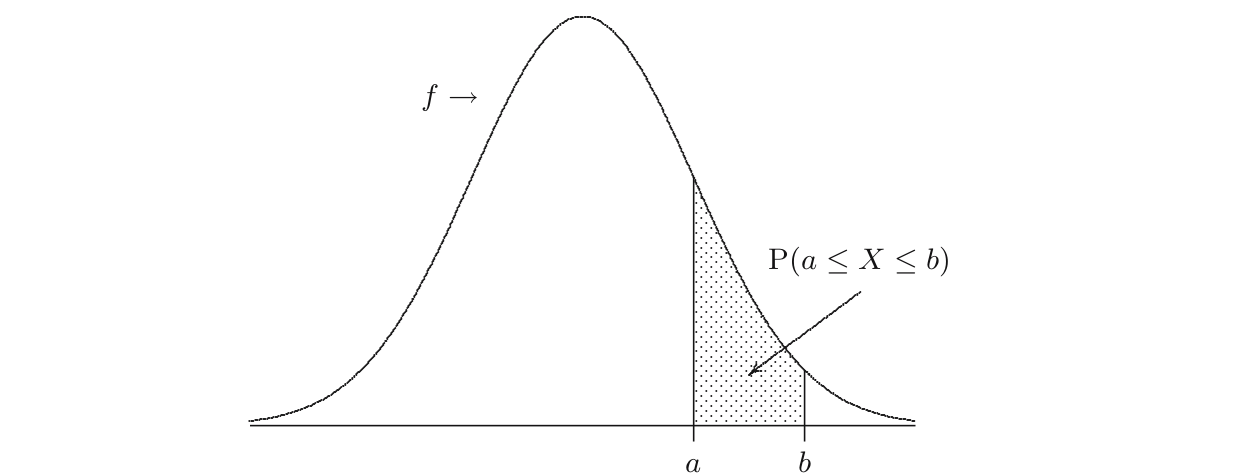
\includegraphics[width=3.64583in,height=\textheight]{sc_1.png}

Definimos al función de distribución acumulada, del mismo modo que
hicimos con variables discretas, pero usando ahora la integral:

\[F(x)=P(X\leq x)=\int _{-\infty }^{x}f(t)\,dt\]

\hypertarget{esperanza-matemuxe1tica}{%
\subsection{Esperanza matemática}\label{esperanza-matemuxe1tica}}

Para una variable aleatoria continua X con función de densidad
\(\displaystyle f(x)\) \textbf{el valor esperado o esperanza matemática}
se define como la integral

\[\displaystyle \operatorname {E} [X]=\int^{\infty}_{-\infty }xf(x)dx\]

Si recordamos es la misma idea que con variable continua, pero en vez de
sumar integramos

\hypertarget{la-distribuciuxf3n-uniforme}{%
\subsection{La distribución
uniforme}\label{la-distribuciuxf3n-uniforme}}

Una variable aleatoria continua tiene una distribución uniforme en el
intervalo \([\alpha, \beta]\) si función de densidad es la siguiente

\[f(x)=\begin{cases}{\frac {1}{b-a}}&\mathrm {para} \ a\leq x\leq b,\\[8pt]0&\text {para el resto de valores}\end{cases}\]

Se denota por \(U(\alpha, \beta)\).

Si calculamos la distribución acumulada:

\[F(x)= \int _{-\infty }^{x}f(t)\,dt\]

veremos que el resultado es

\[\displaystyle F(x)=\begin{cases}0&{\text{para }}x<a\\[8pt]{\frac {x-a}{b-a}}&{\text{para }}a\leq x\leq b\\[8pt]1&{\text{para }}x>b\end{cases}\]

En la siguiente gráfica vemos el ejemplo de la función de masa de una
variable uniforme en \([0,1/3]\)

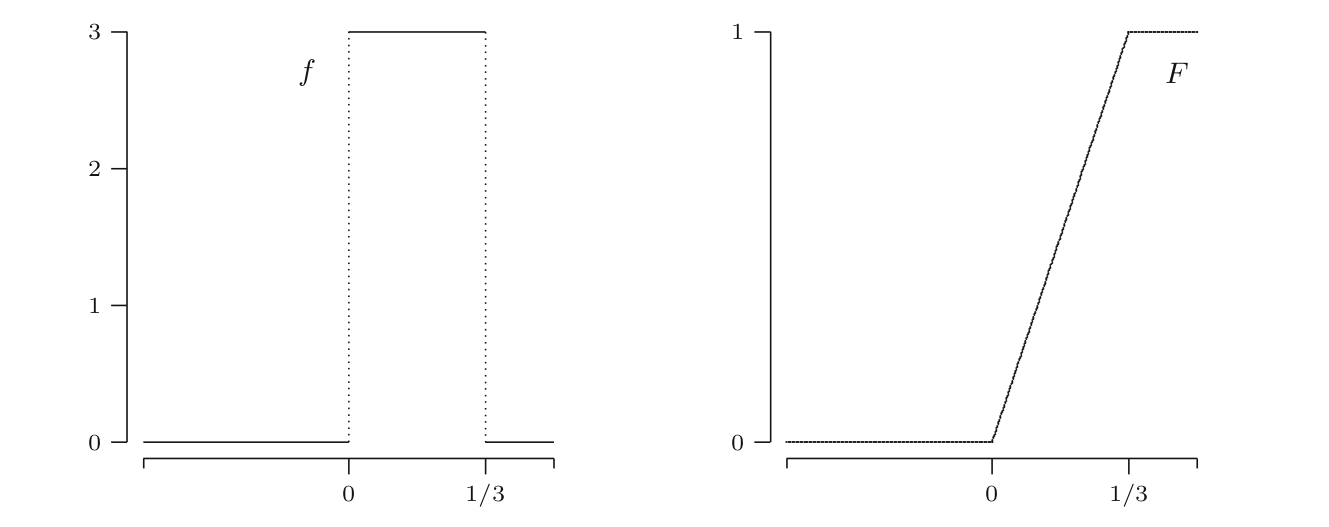
\includegraphics[width=3.64583in,height=\textheight]{sc_2.png}

\hypertarget{la-distribuciuxf3n-normal}{%
\subsection{La distribución normal}\label{la-distribuciuxf3n-normal}}

La distribución normal juega un rol central en la teoría de la
probabilidad y la estadística. Una de sus aplicaciones se debe a C.F.
Gauss, que la usó en 1809 para medir errores en astronomía.

Una función aleatoria continua tiene una \textbf{distribución normal}
con parámetros \(\mu\) y \(\sigma\), su función de densidad de
probabilidad es

\[f(x) = \frac{1}{\sigma \sqrt{2\pi}} e^{-\frac{(x-\mu)^2}{2\sigma^2}}\]

Esta distribución se denota por \(N(\mu, \sigma)\).

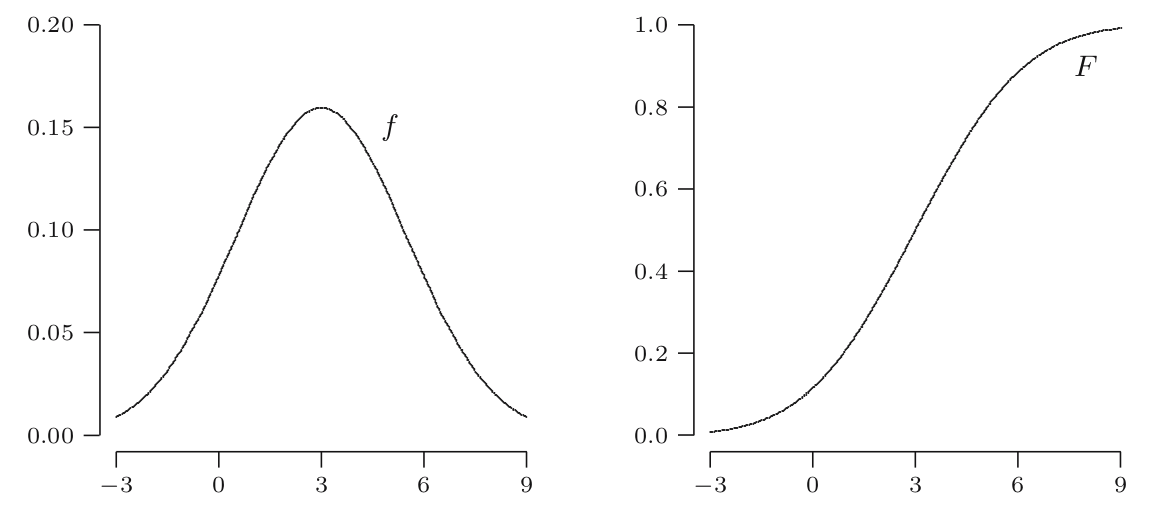
\includegraphics[width=3.64583in,height=\textheight]{sc_3.png}

Como vemos esta función \(f\) tiene una forma de campana, donde los
parámetros \(\mu\) y \(\sigma\) se interpretan como:

\begin{itemize}
\tightlist
\item
  \(\mu\) determina el valor entorno al que se centra la campana.
  Veremos que coincide con la esperanza matemáticas.
\item
  \(\sigma\) determina lo \emph{apretada} que está la campana, es decir
  lo dispersa que está la variable.
\end{itemize}

En la siguiente gráfica vemos la normal para distintos valores de
\(\mu\) y \(\sigma\)

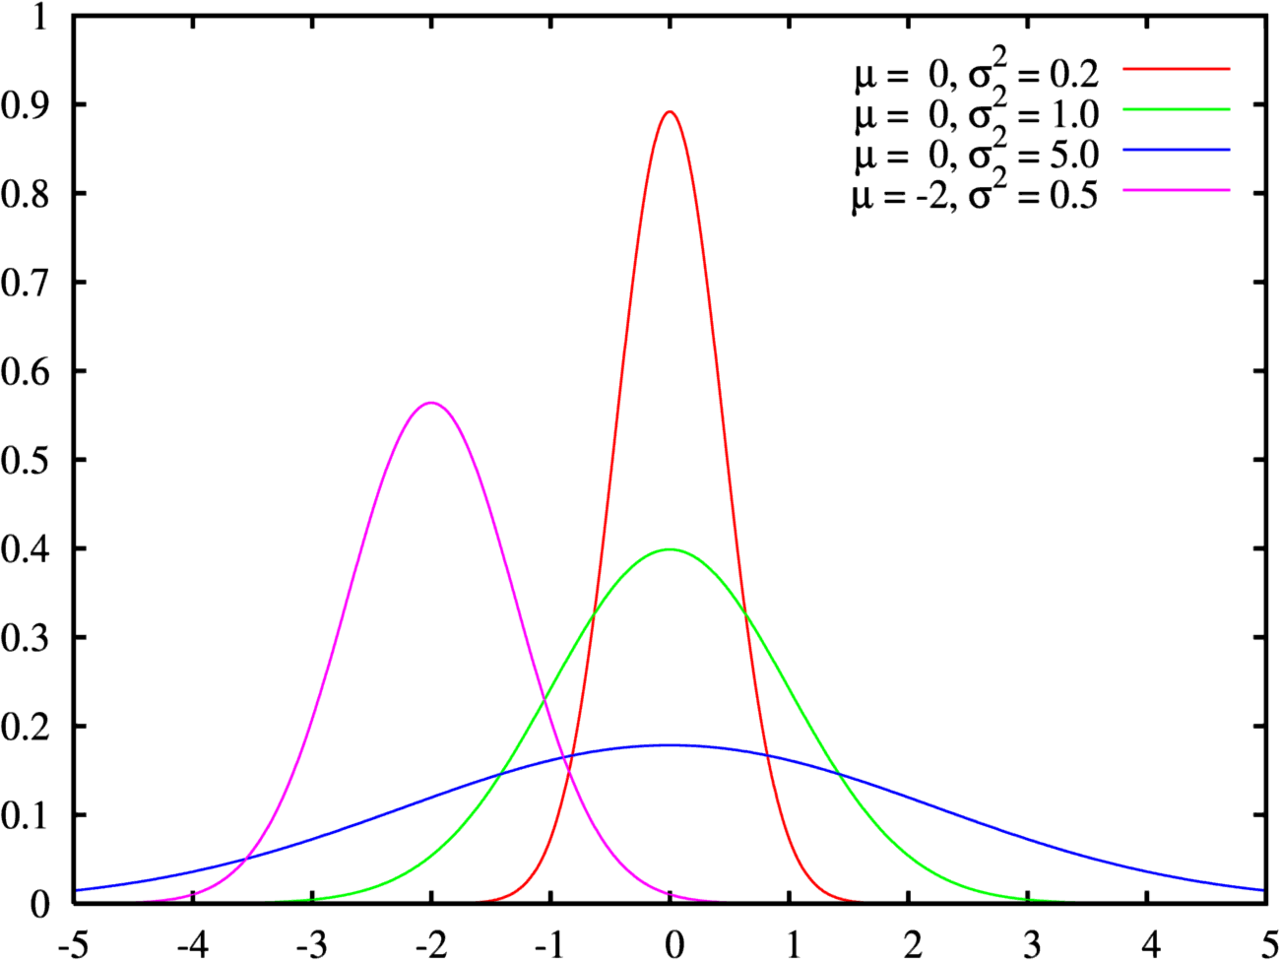
\includegraphics[width=3.64583in,height=\textheight]{normal2.png}

Algunos ejemplos de variables asociadas a fenómenos naturales que siguen
el modelo de la normal son:

\begin{itemize}
\tightlist
\item
  caracteres morfológicos de individuos como la estatura;
\item
  caracteres fisiológicos como el efecto de un fármaco;
\item
  caracteres sociológicos como el consumo de cierto producto por un
  mismo grupo de individuos;
\item
  caracteres psicológicos como el cociente intelectual;
\item
  nivel de ruido en telecomunicaciones;
\item
  errores cometidos al medir ciertas magnitudes;
\end{itemize}

\hypertarget{bibliografuxeda}{%
\section{Bibliografía}\label{bibliografuxeda}}

\begin{itemize}
\tightlist
\item
  John A. Rice. Mathematical Statistics and Data Analysis
\item
  F. M. Dekking, C. Kraailkamp, H. P. Lopuhaa, L. E. Meester. A Modern
  Introduction to Probability and Statistics. Understanding Why and How.
\item
  \url{https://es.wikipedia.org/wiki/Distribuci\%C3\%B3n_Bernoulli}
\item
  \url{https://es.wikipedia.org/wiki/Distribuci\%C3\%B3n_binomial}
\item
  \url{https://es.wikipedia.org/wiki/Distribuci\%C3\%B3n_geom\%C3\%A9trica}
\end{itemize}

\end{document}